\documentclass{article}
\usepackage[utf8]{inputenc}
\usepackage{pgfplots,multicol}
\usepackage{tikz-qtree}
\usepackage{url}
\usepackage{hyperref}
\usepackage{xcolor}
\usepackage{avm}
\usepackage{forest}
\useforestlibrary{linguistics}
\forestapplylibrarydefaults{linguistics}
\hypersetup{
  colorlinks   = true, %Colours links instead of ugly boxes
  urlcolor     = red, %Colour for external hyperlinks
  linkcolor    = blue, %Colour of internal links
  citecolor   = blue %Colour of citations
}
\pgfplotsset{compat=newest} 
\newcommand{\textarray}[1]{\ensuremath{\left[ \mbox{\ttfamily\begin{tabular}{l} #1 \end{tabular}}\right]}}
\begin{document}
\title{566 HW1}
\author{Daniel Campos  \tt {dacampos@uw.edu}}
\date{10/02/2019}
\maketitle 
\section{Chapter 2 Problem 2}
Show that the grammar in (23) can account for the ambiguity of each of the following
sentences by providing at least two trees licensed for each one, and explain briefly which
interpretation goes with which tree. \\
S - NP VP \\
NP - (D) NOM \\
VP - V (NP) (NP) \\
NOM - N \\
NOM - NOM PP \\
VP - VP PP \\
PP - P NP \\
X - X+ CONJ X \\
Note: the tree software I used required turning each node into one word so nouns with multiple words become one word(E.G. Wonder Woman to WonderWoman).
\subsection{Bo saw the group with the telescope.}
Two possible interpretations are that Bo saw a group that had a telescope and Bo saw a group with a telescope. In Figure  \ref{fig:1}, the group that was viewed has a telescope while in Figure  \ref{fig:2} the group was seen with a telescope.
\subsection{Most dogs and cats with fleas live in this neighborhood.}
Two possible trees can revolve around who has flees. Figure  \ref{fig:3} parses the sentence as both the dogs and cats having fleas while Figure  \ref{fig:4} only the cats have fleas.
\subsection{The pictures show Superman and Lois Lane and Wonder Woman.}
The main distinction in this sentence could be around who were in pictures together. Since there are multiple pictures we can take a bunch of possible intepretations, such as Figure  \ref{fig:5} where there could be a picture containing Superman and Lois Lane and separatley a picture of Wonder Woman or Figure  \ref{fig:6} where there is a picture of Superman and separatley a picture of Lois Lane and Wonder Woman together.
\\
\section{Chapter 3 Problem 3}
The Chapter 3 grammar declares AGR to be a feature appropriate for the types noun,
verb, and det, but so far we haven’t discussed agreement involving determiners. Unlike
the determiner the, most other English determiners do show agreement with the nouns
they combine with:\\
(i) a bird/*a birds \\
(ii) this bird/*this birds \\
(iii) that bird/*that birds\\
(iv) these birds/*these bird\\
(v) those birds/*those bird\\
(vi) many birds/*many bird \\
\subsection{Formulate lexical entries for this and these}
\begin{avm} \< this  , \[{\it word}\\
                                              HEAD & \[{\it DETERMINER}\\
                                                       AGR &\[PER & 1st\\
                                                              NUM & sg\]\]\\
                                              VAL & \[ COMPS & itr\\
  					               SPR & $+$\]\] \> \end{avm}
\\
\begin{avm} \< these  , \[{\it word}\\
                                              HEAD & \[{\it DETERMINER}\\
                                                       AGR &\[PER & 1st\\
                                                              NUM & pl\]\]\\
                                              VAL & \[ COMPS & itr\\
  					               SPR & $+$\]\] \> \end{avm}
\subsection{Modify Head-Specifier Rule 2}
\begin{avm} \[{\it phrase}\\
VAL & \[ COMPS & itr\\
         SPR & $+$\]\] \ $\rightarrow$\ \ {\HD}\[{\it DETERMINER}\\
                                        HEAD & [AGR [NUM {\@1} PER {\@2} ]\\
                                        \] \ \ {\HD}\[{\it phrase}\\
                                        HEAD & [{\it noun} \\  AGR & [NUM {\@1}  PER {\@2}]] \\
                                        VAL & \[ SPR & $-$\]\]
\end{avm}
\subsection{Draw Tree for: these birds }
see Figure  \ref{fig:7}
\section{Chapter 3 Problem 5}
The head of a phrase is the element inside the phrase whose properties determine the
distribution of that phrase, i.e. the environments in which it can occur. We say that
nouns head noun phrases, since (ii)-(v) can all show up in the same environments as (i):
e.g. as the specifier of a verb, as a complement of a transitive verb and as the complement
of prepositions like of or on.
(i) giraffes
(ii) tall giraffes
(iii) giraffes with long necks
(iv) all giraffes
(v) all tall giraffes with long necks
On the other hand (vi)–(ix) do not have the same distribution as the phrases in (i)–(v).
(vi) tall
\subsection{which phrase has the same distribution as two hundred}
three hundred
\subsection{Does your answer support treating two or hundred as the head?}
My answer supports treating hundred as the head. I do this since in many ways the two, which could also be a variable n(representing 0-9), is modifying the main node hundred. By having the hundred be the head we ensure that items in the same class/range are licensed in the same way and are not licesed based on their modification. 
\subsection{which phrase has the same distribution as two hundred five?}
Two hundred six.
\subsection{Does your answer to part (C) support treating two hundred or five as the head}
Similair to the previous example, I belive the two hundred should be treated as the head. In this example, the largest unit which is being modified is the hudred denomination and thus it is the head of the phrase. Both the two (of two hundred) and the five and modifying the central unit, hundred, and thus hundred should be the head.
\begin{figure}
 \centering
 \caption{Bo sees a group that has a telescope}
 \label{fig:1}
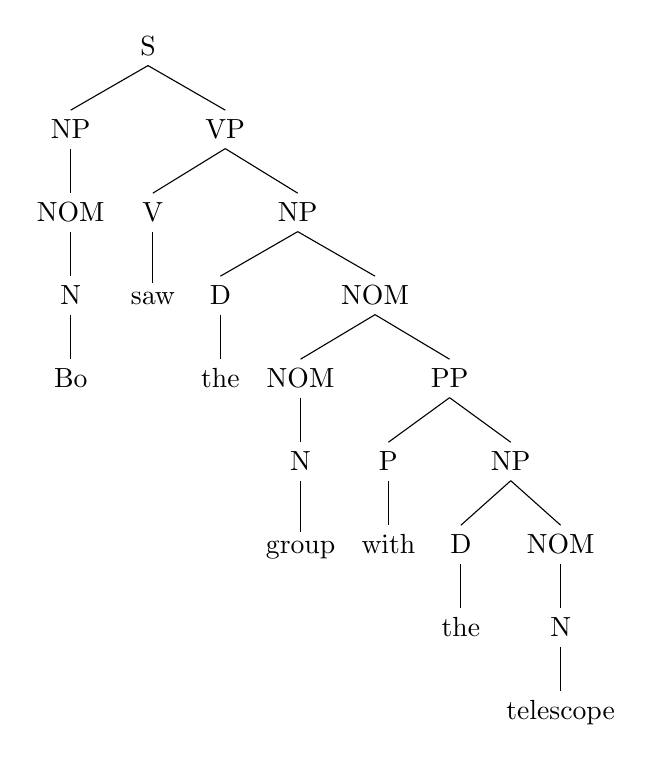
\begin{tikzpicture}[%
  sibling distance=.1cm,
  empty/.style={draw=none},
  tlabel/.style={font=\footnotesize\color{red!70!black}}]
\Tree  
[.S  
	[.NP 
		[.NOM 
			[.N 
				[.Bo ] ] ] ]
	[.VP 
		[.V 
			[.saw ] ]
		[.NP 
			[.D 
				[.the ] ] 
			[.NOM 
				[.NOM 
					[.N 
						[.group ] ] ] 
				[.PP 
					[.P 
						[.with ] ] 
					[.NP 
						[.D 
							[.the ] ] 
						[.NOM 
							[.N
								[.telescope ] ] ] ] ] ] ] ] ]
\end{tikzpicture}
\end{figure}
\begin{figure}
 \centering
 \caption{Bo sees a group using a telescope}
 \label{fig:2}
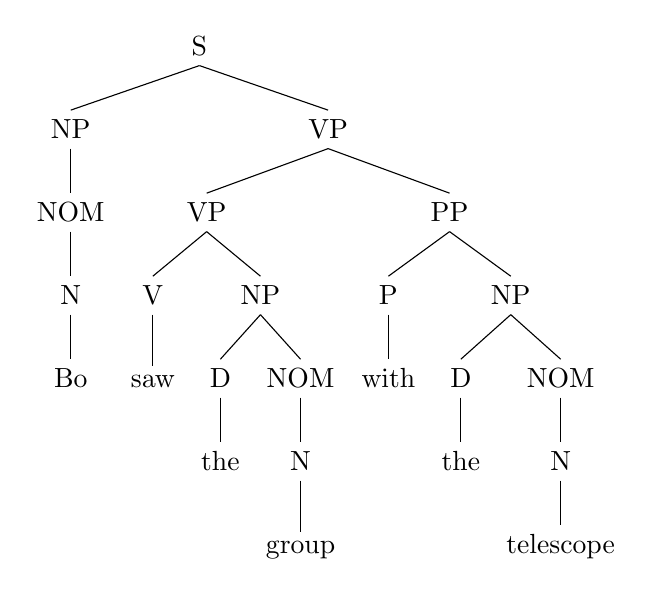
\begin{tikzpicture}[%
  sibling distance=.1cm,
  empty/.style={draw=none},
  tlabel/.style={font=\footnotesize\color{red!70!black}}]
\Tree  
[.S  
	[.NP 
		[.NOM 
			[.N 
				[.Bo ] ] ] ]
	[.VP 
		[.VP 
			[.V 
				[.saw ] ]
		[.NP 
			[.D 
				[.the ] ] 
			[.NOM 
				[.N [.group ] ] ] ] ] 
		[.PP 
			[.P 
				[.with ] ] 
			[.NP 
				[.D 
					[.the ] ] 
				[.NOM 
					[.N
						[.telescope ] ] ] ] ] ] ]
\end{tikzpicture}
\end{figure}
\begin{figure}
 \centering
 \caption{Most dogs and cats with fleas live in this neighborhood where both cats and dogs have fleas}
 \label{fig:3}
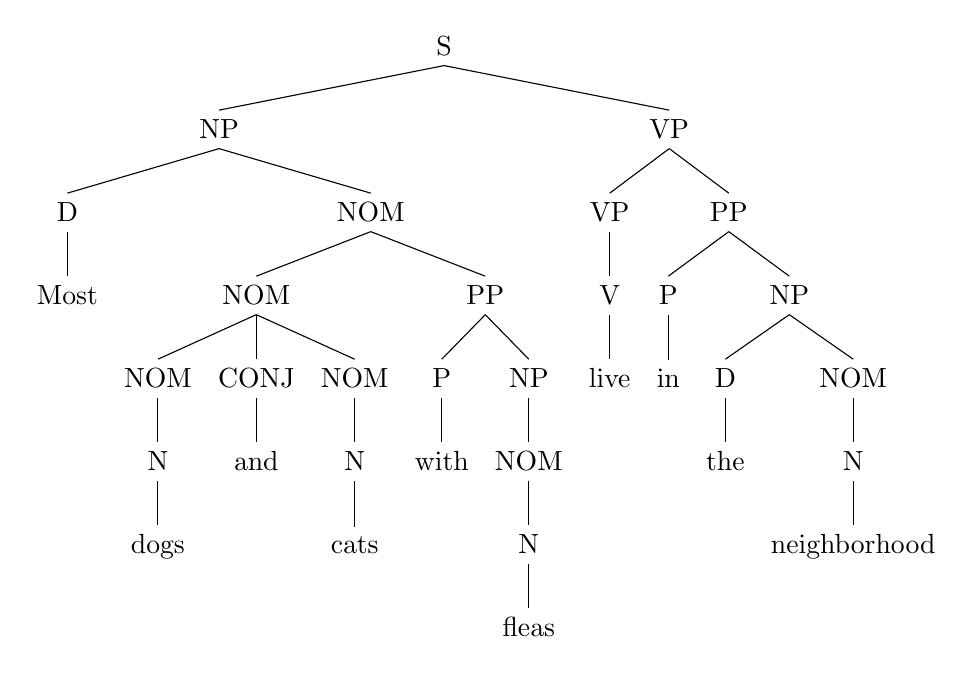
\begin{tikzpicture}[%
  sibling distance=.1cm,
  empty/.style={draw=none},
  tlabel/.style={font=\footnotesize\color{red!70!black}}]
\Tree  
[.S  
	[.NP 
		[.D 
			[.Most ] ]
		[.NOM
			[.NOM 
				[.NOM 
					[.N 
						[.dogs ] ] ]
				[.CONJ 
					[.and ] ] 
                    	[.NOM
					[.N
						[.cats ] ] ] ]  
			[.PP 
				[.P 
					[.with ] ]
				[.NP 
					[.NOM 
						[.N
							[.fleas ] ] ] ] ] ] ]
	[.VP
		[.VP 
			[.V 
				[.live ] ] ]
		[.PP 
			[.P
				[.in ] ]
			[.NP
				[.D
					[.the ] ]
				[.NOM
					[.N
						[.neighborhood ] ] ] ] ] ] ]
\end{tikzpicture}
\end{figure}
\begin{figure}
 \centering
 \caption{Most dogs and cats with fleas live in this neighborhood where only the cats have fleas}
 \label{fig:4}
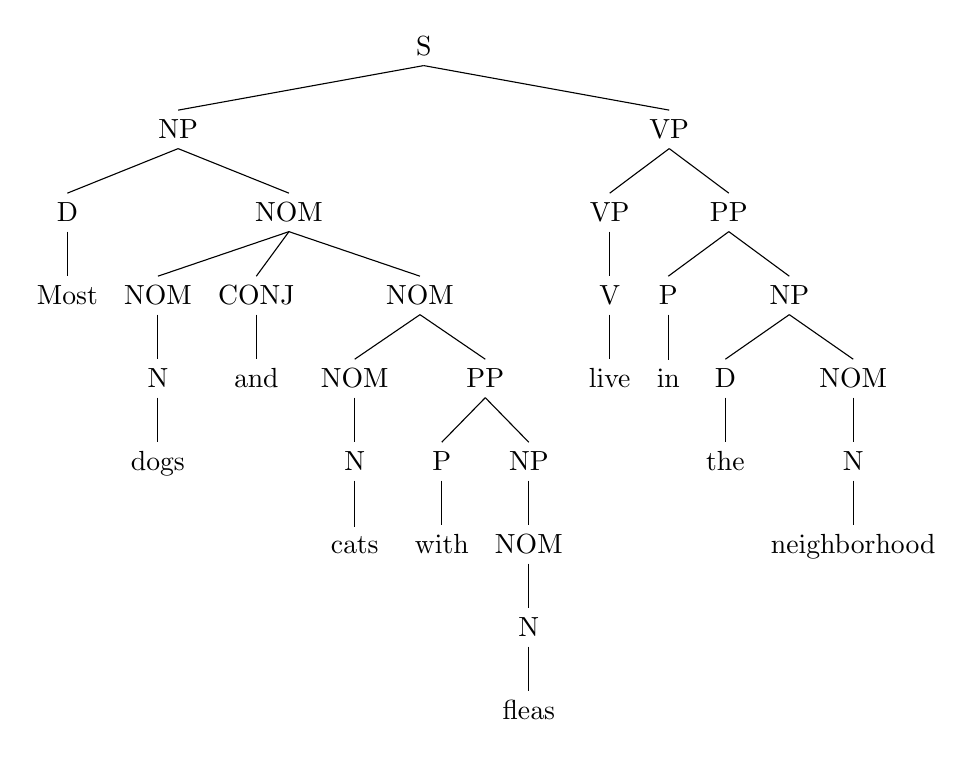
\begin{tikzpicture}[%
  sibling distance=.1cm,
  empty/.style={draw=none},
  tlabel/.style={font=\footnotesize\color{red!70!black}}]
\Tree  
[.S  
	[.NP 
		[.D 
			[.Most ] ]
		[.NOM
			[.NOM 
				[.N 
					[.dogs ] ] ]
			[.CONJ 
				[.and ] ] 
                    [.NOM
				[.NOM
					[.N
						[.cats ] ] ]
				[.PP 
					[.P 
						[.with ] ]
					[.NP 
						[.NOM 
							[.N
								[.fleas ] ] ] ] ] ] ] ]
	[.VP
		[.VP 
			[.V 
				[.live ] ] ]
		[.PP 
			[.P
				[.in ] ]
			[.NP
				[.D
					[.the ] ]
				[.NOM
					[.N
						[.neighborhood ] ] ] ] ] ] ]
\end{tikzpicture}
\end{figure}
\begin{figure}
 \centering
 \caption{The pictures show Superman and Lois Lane together and separatley they also show Wonder Woman}
 \label{fig:5}
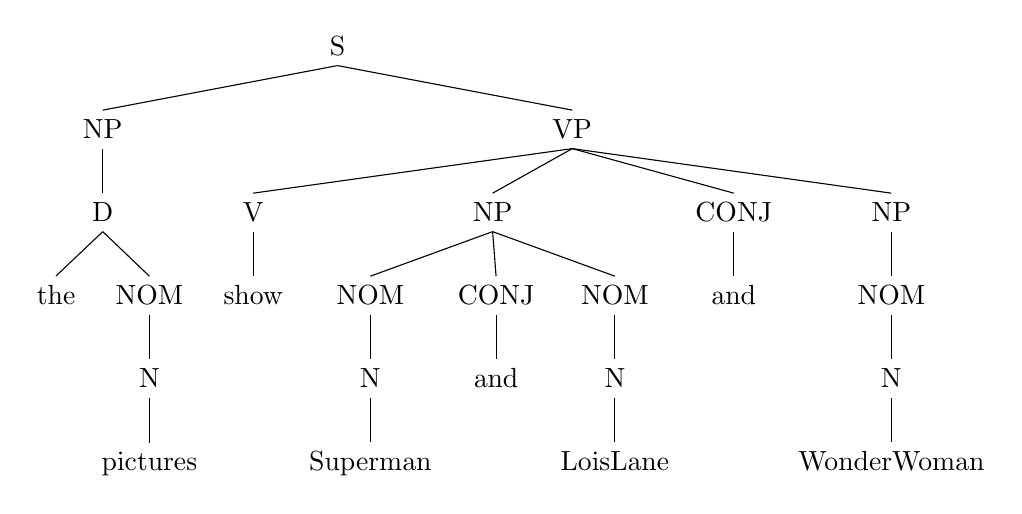
\begin{tikzpicture}[%
  sibling distance=.1cm,
  empty/.style={draw=none},
  tlabel/.style={font=\footnotesize\color{red!70!black}}]
\Tree  
[.S  
	[.NP 
		[.D 
			[.the ]
		[.NOM 
			[.N 
				[.pictures ] ] ] ] ]
	[.VP 
		[.V 
			[.show ] ]
		[.NP 
			[.NOM 
				[.N
					[.Superman ] ] ]
			[.CONJ 
				[.and ] ]
			[.NOM 
				[.N
					[.LoisLane ] ] ] ]
		[.CONJ 
			[.and ] ]
		[.NP 
			[.NOM 
				[.N
					[.WonderWoman ] ] ] ] ] ]
\end{tikzpicture}
\end{figure}
\begin{figure}
 \centering
 \caption{The pictures show Superman and separately Lois Lane and Wonder Woman together}
 \label{fig:6}
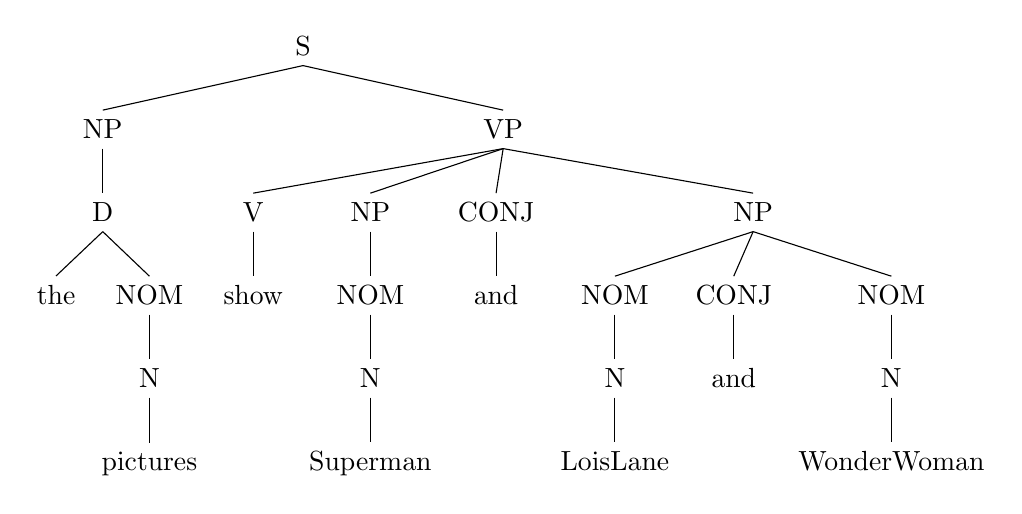
\begin{tikzpicture}[%
  sibling distance=.1cm,
  empty/.style={draw=none},
  tlabel/.style={font=\footnotesize\color{red!70!black}}]
\Tree  
[.S  
	[.NP 
		[.D 
			[.the ]
		[.NOM 
			[.N 
				[.pictures ] ] ] ] ]
	[.VP 
		[.V 
			[.show ] ]
		[.NP 
			[.NOM 
				[.N
					[.Superman ] ] ] ] 
		[.CONJ 
			[.and ] ]
		[.NP
			[.NOM 
				[.N
					[.LoisLane ] ] ]
			[.CONJ 
				[.and ] ]
			[.NOM 
				[.N
					[.WonderWoman ] ] ] ] ] ]
\end{tikzpicture}
\end{figure}
\begin{figure}
 \centering
 \caption{These Birds}
 \label{fig:7}
\begin{forest}
[S \textarray{phrase \\ HEAD noun \\ \textarray{AGR  \textarray{PER 1st \\ NUM pl}}}
[NP phrase \textarray{HEAD noun \\ \textarray{AGR \textarray{PER 1st \\ NUM pl}}}
[D \textarray{HEAD det \\ \textarray{PER 1st \\ NUM pl}} [these ]] 
[N \textarray{HEAD noun \\ \textarray{PER 1st \\ NUM pl}} [birds]]]]
\end{forest}
\end{figure}
\end{document}
